\documentclass{article}
\usepackage[margin=0.5in]{geometry}
\usepackage{amsmath}
\usepackage{graphicx}
\usepackage{amssymb}
\usepackage{multicol}
\usepackage{xcolor}
\usepackage{amsthm}
\usepackage{mdframed}

\newenvironment{tightcenter}{%
    \setlength\topsep{0pt}
    \setlength\parskip{0pt}
    \begin{center}
}{%  
    \end{center}
}
\newcommand{\R}{\mathbb{R}}
\newcommand{\Z}{\mathbb{Z}}
\newcommand{\C}{\mathbb{C}}
\newcommand{\K}{\mathbb{K}}
\newcommand{\PP}{\mathbb{P}}
\newcommand{\E}{\mathcal{E}}
\title{Trabajo Práctico 4 - Representación matricial de transformaciones lineales}
\author{Santiago}
\date{}
\begin{document}
    \maketitle
    \global\mdfdefinestyle{s}{%
            linecolor=orange,linewidth=0.5pt,%
            leftmargin=0cm,rightmargin=1cm
        }
    \begin{enumerate}
        \item Considerar las transformaciones lineales $R_{\frac{\pi}{2}},S_Y,H_2$ y $P_X$ del ejercicio 11 de la práctica 2 y escribir su representación matricial con respecto a la base $B=\{(1,1),(1,-1)\}$
    \begin{mdframed}[style=s]
        \begin{itemize}
            \item $R_\frac{\pi}{2}(x,y)=(-y,x)$
                \begin{center}
                    $[R_\frac{\pi}{2}]_B=\left([R_\frac{\pi}{2}(1,1)]_B\quad[R_\frac{\pi}{2}(1,-1)]_B\right)$\\
                    $\to [R_\frac{\pi}{2}]_B=\begin{pmatrix}
                        0&1\\-1&0
                    \end{pmatrix}$
                \end{center}
                Si tomamos un vector arbitrario de $\R^2$, la transformación lo afecta de la siguiente manera
                \[[R_\frac{\pi}{2}]_B[v]_B=\begin{pmatrix}
                    0&1\\-1&0
                \end{pmatrix}\begin{pmatrix}
                    \alpha\\\beta
                \end{pmatrix}=\begin{pmatrix}
                    -\beta\\\alpha
                \end{pmatrix}\]
                En la Figura 1 se observa la transformación de dos vectores.
                \begin{center}
                    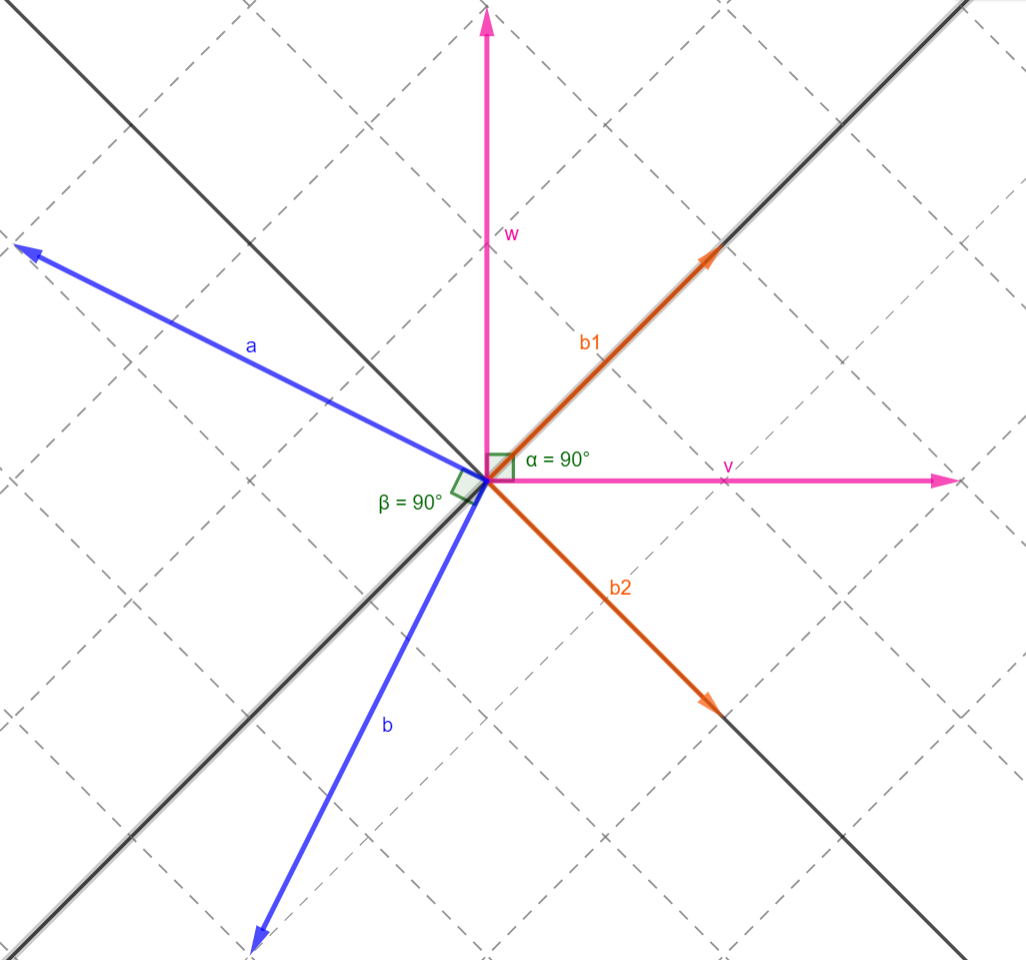
\includegraphics[width=0.4\textwidth]{Img/Ej1a.png}\\
                    Figura 1. Transformación bajo $R_\frac{\pi}{2}$ de $v$ y $a$ en el sistema de coordenadas $B$.
                \end{center}
            \item $S_Y(x,y)=(-x,y)$
                \begin{center}
                    $[S_Y]_B=\left([S_Y(1,1)]_B\quad[S_Y(1,-1)]_B\right)$\\
                    $\to [S_Y]_B=\begin{pmatrix}
                        0&-1\\-1&0
                    \end{pmatrix}$
                \end{center}
                En la Figura 2 se observan las transformaciones de los mismos dos vectores de la Figura 1, ahora bajo $S_Y$
                \begin{center}
                    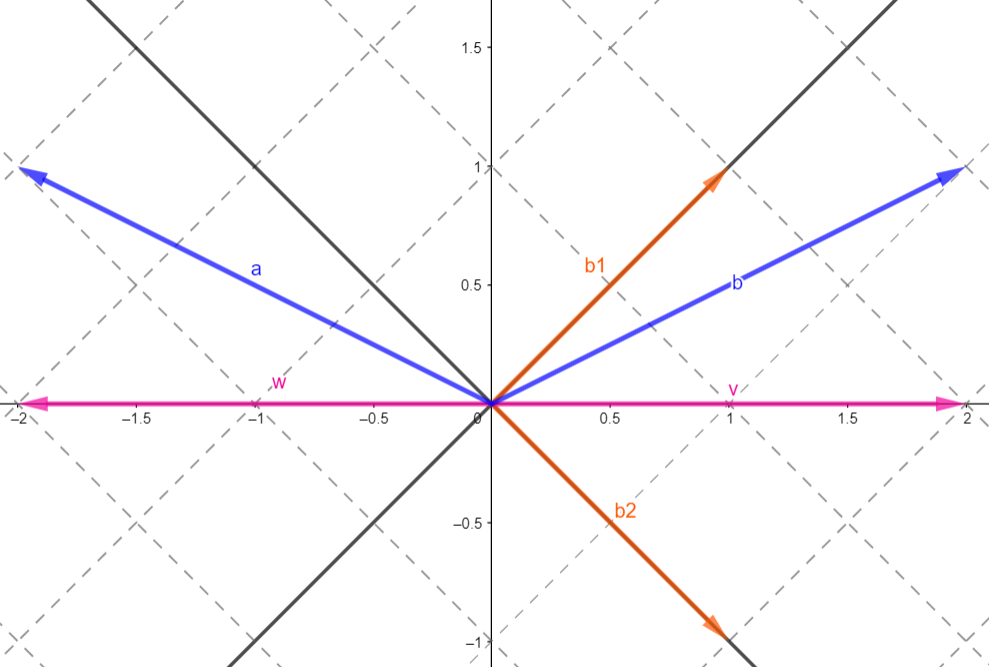
\includegraphics[width=0.4\textwidth]{Img/Ej1a2.png}\\
                    Figura 2. Transformación bajo $S_Y$ de $v$ y $a$ en el sistema de coordenadas $B$.
                \end{center}
            \item $H_2(x,y)=(2x,2y)$
                \begin{center}
                    $[H_2]_B=\left([H_2(1,1)]_B\quad[H_2(1,-1)]_B\right)$\\
                    $\to [H_2]_B=\begin{pmatrix}
                        2&0\\0&2
                    \end{pmatrix}$
                \end{center}
                En la Figura 3, se observa esta transformación.
                \begin{center}
                    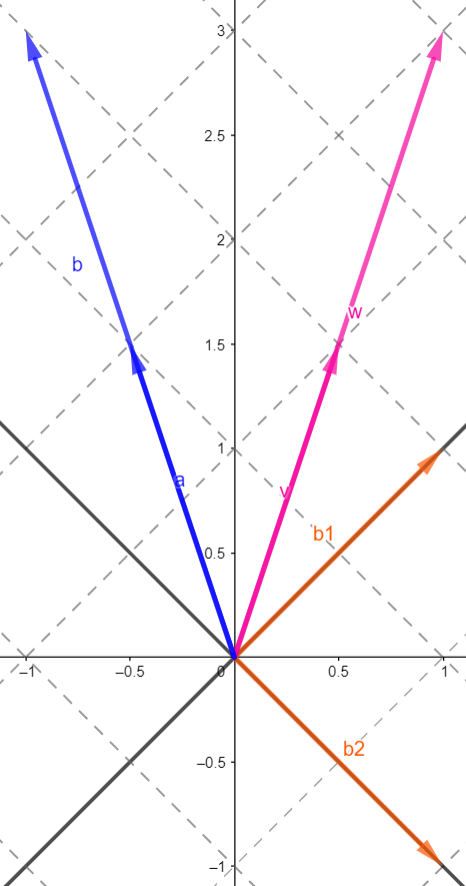
\includegraphics[width=0.2\textwidth]{Img/Ej1a3.png}\\
                    Figura 3. Transformación bajo $H_2$ de $v$ y $a$ en el sistema de coordenadas $B$.
                \end{center}
                Un dato a tener en cuenta es que \[[H_2]_B=\begin{pmatrix}
                    2&0\\0&2
                \end{pmatrix}=[H_2]_\E\]
                Supongamos el caso de la transformación más general: $H_k$ y supongamos una base cualquiera de $\R^2$, denominada $\tilde{B}=\{b_1,b_2\}$. Si quiero encontrar la representación matricial de $H_k$ en la base $\tilde{B}$:\[[H_k]_{\tilde{B}}=\left([H_k(b1)]_{\tilde{B}}\quad[H_k]_{\tilde{B}}\right)=\left([kb_1]_{\tilde{B}}\quad[kb_2]_{\tilde{B}}\right)=\begin{pmatrix}
                    k&0\\0&k
                \end{pmatrix}\]
                Por lo tanto, la representación matricial en cualquier base es la misma.¿Se puede sacar alguna conclusión de esto?
            \item $P_X(x,y)=(x,0)$
                \begin{center}
                    $[P_X]_B=\left([P_X(1,1)]_B\quad[P_X(1,-1)]_B\right)$\\
                    $\to [P_X]_B=\begin{pmatrix}
                        1/2&1/2\\1/2&1/2
                    \end{pmatrix}$
                \end{center}
        \end{itemize}
    \end{mdframed}
        \item Sea $T:\R^3\to\R^3$, la transformación lineal dada por $T(x,y,z)=(z,y+z,x+y+z)$.
    \begin{enumerate}
        \item Hallar la reprenstación matricial de $T$ con respecto a la base canónica de $\R^3$.
            \begin{mdframed}[style=s]
                \begin{center}
                    $[T]_\E=\left([T(1,0,0)]_\E\quad[T(0,1,0)]_\E\quad[T(0,0,1)]_\E\right)$\\
                    $[T]_\E=\begin{pmatrix}
                        0&0&1\\0&1&1\\1&1&1
                    \end{pmatrix}$
                \end{center}
            \end{mdframed}
        \item Sea $B=\{(1,1,0),(1,2,3),(1,3,5)\}$. Hallar las matrices de cambio de base $P_{\E,B}$ y $P_{B,\E}$
            \begin{mdframed}[style=s]
                Para encontrar $P_{\E,B}$ tenemos que
                \begin{center}
                    $P_{\E,B}=\left([(1,1,0)]_\E\quad[(1,2,3)]_\E\quad[(1,3,5)]_\E\right)$\\
                    $\to P_{\E,B}=\begin{pmatrix}
                        1&1&1\\1&2&3\\0&3&5
                    \end{pmatrix}$
                \end{center}
                Mientras que
                \begin{center}
                    $P_{B,\E}=\left([(1,0,0)]_B\quad[(0,1,0)]_B\quad[(0,0,1)]_B\right)$\\
                    $\to P_{B,\E}=\begin{pmatrix}
                        -1&2&-1\\5&-5&2\\-3&3&-1
                    \end{pmatrix}$
                \end{center}
            \end{mdframed}
        \item Hallar la reprenstación matricial de $T$ con respecto a la base $B$.
            \begin{mdframed}[style=s]
                \begin{center}
                    $[T]_B=\left([T(1,1,0)]_B\quad[T(1,2,3)]_B\quad[T(1,3,5)]_B\right)$\\
                    $\begin{cases}
                        [T(1,1,0)]_B=[(0,1,2)]_B=P_{B,\E}\cdot(0,1,2)^T\\
                        [T(1,2,3)]_B=[(3,5,6)]_B=P_{B,\E}\cdot(3,5,6)^T\\
                        [T(1,3,5)]_B=[(5,8,9)]_B=P_{B,\E}\cdot(5,8,9)^T
                    \end{cases}$\\
                    $\to [T]_B=\begin{pmatrix}
                        0&1&2\\1&2&3\\1&-6&0
                    \end{pmatrix}$
                \end{center}
            \end{mdframed}
    \end{enumerate}
        \item Sea $T:\R^2\to\R^3$, la transformación lineal dada por $T(x,y)=(3x+y,-y,x+y)$. Consideremos $B=\{(1,1),(-1,0)\}$ y $\tilde{B}=\{(1,0,1),(1,-1,0),(0,2,1)\}$, bases de $\R^2$ y $\R^3$, respectivamente. Hallar la matriz $[T]_{\tilde{B},B}$, es decir, la matriz de la transformación $T$ con respecto a las bases $B$ y $\tilde{B}$.
    \begin{mdframed}[style=s]
        \begin{center}
            $[T]_{\tilde{B},B}=\left([T(1,1)]_{\tilde{B}}\quad[T(-1,0)]_{\tilde{B}}\right)=\left([(4,-1,2)]_{\tilde{B}}\quad[(-3,0,-1)]_{\tilde{B}}\right)$
        \end{center}
        Para hallar las coordenadas de un vector en la base $\tilde{B}$, calculo $P_{\tilde{B},\E}$
        \[P_{\tilde{B},\E}=\left([(1,0,0)]_{\tilde{B}}\quad[(0,1,0)]_{\tilde{B}}\quad[(0,0,1)]_{\tilde{B}}\right)=\begin{pmatrix}
            -1&-1&2\\2&1&-2\\1&1&-1
        \end{pmatrix}\]
        Entonces,
        \begin{center}
            $\begin{cases}
                [4,-1,2]_{\tilde{B}}=P_{\tilde{B},\E}\cdot(4,-1,2)^T=(1,3,1)\\
                [-3,0,-1]_{\tilde{B}}=P_{\tilde{B},\E}\cdot(-3,0,-1)^T=(1,-4,-2)
            \end{cases}$
        \end{center}
        Por lo tanto,
        \[[T]_{\tilde{B},B}=\begin{pmatrix}
            1&1\\3&-4\\1&-2
        \end{pmatrix}\]
    \end{mdframed}
        \item Sea $T:\R^3\to\R^3$, la transformación lineal dada por $T(x,y,z)=(2y+z,x-4y,3x)$.
    \begin{enumerate}
        \item Hallar $[T]_B$ para la base $B=\{(1,1,1);(1,1,0);(1,0,0)\}$ de $\R^3$.
            \begin{mdframed}[style=s]
                \begin{center}
                    $[T]_B=\left([T(1,1,1)]_B\quad[(1,1,0)]_B\quad[(1,0,0)]_B\right)$\\
                    $\to [T]_B=\begin{pmatrix}
                        3&3&3\\-6&-6&-2\\6&5&-1
                    \end{pmatrix}$
                \end{center}
            \end{mdframed}
        \item Probar que $[T(v)]_B=[T]_B[v]_B$, para $v\in\R^3$.
            \begin{mdframed}[style=s]
                Por un lado se tiene que
                \[[T(v)]_B=[T(x,y,z)]_B=[(2y+z,x-4y,3x)]_B=\begin{pmatrix}
                    3x\\-2x-4y\\-x+6y+z
                \end{pmatrix}\]
                Por el otro lado
                \[[T]_B[v]_B=\begin{pmatrix}
                    3&3&3\\-6&-6&-2\\6&5&-1
                \end{pmatrix}\begin{pmatrix}
                    z\\y-z\\x-y
                \end{pmatrix}=\begin{pmatrix}
                    3x\\-2x-4y\\-x+6y+z
                \end{pmatrix}\]
            \end{mdframed}
    \end{enumerate}
        \item Sea $T:\C^2\to\C^2$ la transformación lineal dada por $T(x,y)=(y,0)$. Consideremos la base $B=\{(1,i),(-i,2)\}$ de $\C^2$ como $\C$-EV.
    \begin{enumerate}
        \item Hallar la representación matricial de $T$ con respecto a las bases $\E$ y $B$.\pagebreak
            \begin{mdframed}[style=s]
                \begin{center}
                    $[T]_{B,\E}=\left([T(1,0)]_B\quad[T(0,1)]_B\right)$\\
                    $\to [T]_{B,\E}=\begin{pmatrix}
                        0&2\\0&-i
                    \end{pmatrix}$
                \end{center}
            \end{mdframed}
        \item Hallar la representación matricial de $T$ con respecto a las bases $B$ y $\E$.
            \begin{mdframed}[style=s]
                \begin{center}
                    $[T]_{\E,B}=\left([T(1,i)]_\E\quad[T(-i,2)]_\E\right)$\\
                    $\to [T]_{\E,B}=\begin{pmatrix}
                        1&-i\\i&2
                    \end{pmatrix}$
                \end{center}
            \end{mdframed}
        \item Hallar la representación matricial de $T$ con respecto a la base $B$. Calcular el determinante y la traza.
            \begin{mdframed}[style=s]
                \begin{center}
                    $[T]_B=\left([T(1,i)]_B\quad[T(-i,2)]_B\right)$\\
                    $\to [T]_B=\begin{pmatrix}
                        2i&4\\1&-2i
                    \end{pmatrix}$\\
                    $tr([T]_B)=0\qquad det([T]_B)=0$
                \end{center}
            \end{mdframed}
        \item Elegir otra base de $\C^2$ y hallar la representación matricial de $T$ con respecto a esa base. ¿Puede decir cuánto valen el determinante y la traza sin hacer las cuentas? Justificar.
            \begin{mdframed}[style=s]
                Propongo $\tilde{B}=\{(i,0),(0,1)\}$
                \begin{center}
                    $[T]_{\tilde{B}}=\left([T(i,0)]_{\tilde{B}}\quad[T(0,1)]_{\tilde{B}}\right)$\\
                    $\to [T]_{\tilde{B}}=\begin{pmatrix}
                        0&-i\\0&0
                    \end{pmatrix}$
                \end{center}
                La traza y el determinante son propias de la transformación, así que no importa la base, el resultado siempre será el mismo.
            \end{mdframed}
    \end{enumerate}
        \item Consideremos a $\C$ como un $\R$-EV y sea $T:\C\to\C$ dada por $T(z)=\bar{z}$.
    \begin{enumerate}
        \item Probar que $T$ es una transformación lineal.
            \begin{mdframed}[style=s]
                Sean $\alpha\in\R,u,v\in\C$
                \begin{align*}
                    T(\alpha u+v)&=\overline{\alpha u+v}\\
                    &=\overline{\alpha u}+\overline{v}\\
                    &=\overline{\alpha}\overline{u}+\overline{v}\\
                    &=\alpha \overline{u}+\overline{v}\\
                    &=\alpha T(u)+T(v)
                \end{align*}
                Por lo tanto, $T$ es una transformación lineal.
            \end{mdframed}
        \item Hallar la representación matricial $[T]_B$ para la base $B=\{1,i\}$ y $[T]_{\tilde{B}}$ para la base $\tilde{B}=\{1+i,1-i\}$.
            \begin{mdframed}[style=s]
                \begin{center}
                    $\begin{cases}
                        [T]_B=\left([T(1)]_B\quad[T(i)]_B\right)&\to[T]_B=\begin{pmatrix}
                            1&0\\0&-1
                        \end{pmatrix}\\
                        [T]_{\tilde{B}}=\left([T(1+i)]_{\tilde{B}}\quad[T(1-i)]_{\tilde{B}}\right)&\to[T]_{\tilde{B}}=\begin{pmatrix}
                            0&1\\1&0
                        \end{pmatrix}
                    \end{cases}$
                \end{center}
            \end{mdframed}
        \item Hallar $P_{B,\tilde{B}}$ y $P_{\tilde{B},B}$.
            \begin{mdframed}[style=s]
                \[\begin{cases}
                    P_{B,\tilde{B}}=\left([(1+i)]_B\quad[(1-i)]_B\right)&=\begin{pmatrix}
                        1&1\\1&-1
                    \end{pmatrix}\\
                    P_{\tilde{B},B}=\left([(1)]_{\tilde{B}}\quad[(i)]_{\tilde{B}}\right)&=\begin{pmatrix}
                        1/2&1/2\\1/2&-1/2
                    \end{pmatrix}
                \end{cases}\]
            \end{mdframed}
        \item Probar que $[T]_{\tilde{B}}=P_{\tilde{B},B}[T]_BP_{B,\tilde{B}}$,
            \begin{mdframed}[style=s]
                \[P_{\tilde{B},B}[T]_BP_{B,\tilde{B}}=\begin{pmatrix}
                    1/2&1/2\\1/2&-1/2
                \end{pmatrix}\begin{pmatrix}
                    1&0\\0&-1
                \end{pmatrix}\begin{pmatrix}
                    1&1\\1&-1
                \end{pmatrix}=\begin{pmatrix}
                    0&1\\1&0
                \end{pmatrix}\]
                Con lo cual se demuestra la igualdad.
            \end{mdframed}
    \end{enumerate}
        \item Sea $T:\R^2[x]\to\R^3$, la transformación lineal dada por \[T(ax^2+bx+c)=(a+2b+c,a+b,2a+b-c).\]
    \begin{enumerate}
        \item Hallar una representación matricial de $T$.
            \begin{mdframed}[style=s]
                La más sencilla que se me ocurre es con respecto a $\E=\{(1,0,0),(0,1,0),(0,0,1)\}$ y $B=\{1,x,x^2\}$
                \begin{center}
                    $[T]_{\E,B}=\left([T(1)]_\E\quad[T(x)]_\E\quad[T(x^2)]_\E\right)$\\
                    $\to [T]_{\E,B}=\left([(1,0,-1)]_\E\quad[(2,1,1)]_\E\quad[(1,1,2)]_\E\right)$\\
                    $\to [T]_{\E,B}=\begin{pmatrix}
                        1&2&1\\0&1&1\\-1&1&2
                    \end{pmatrix}$ 
                \end{center}
            \end{mdframed}
        \item Hallar la dimensión del núcleo y de la imagen.
            \begin{mdframed}[style=s]
                $N(T)=\{p\in\R_2[x]:T(p)=(0,0,0)\}$. Si $p(x)=ax^2+bx+c$. Entonces, me fijo en resolver
                \begin{center}
                    $\begin{pmatrix}
                        1&2&1\\0&1&1\\-1&1&2
                    \end{pmatrix}\begin{pmatrix}
                        c\\b\\a
                    \end{pmatrix}=\begin{pmatrix}
                        0\\0\\0
                    \end{pmatrix}\to\begin{cases}
                        c+2b+a=0\\
                        b+a=0\\
                        -c+b+2a=0
                    \end{cases}\to\begin{cases}
                        b=-a\\
                        c=a
                    \end{cases}\to p(x)=a(x^2-x+1)$
                \end{center}
                Por lo tanto, se tiene que\[N(T)=\overline{\{x^2-x+1\}}\to dim(N(T))=1\]
                Por el teorema de la dimensión:
                \[dim(Im(T))=2\]
            \end{mdframed}
        \item Sea $W$ un subespacio de $\R^3$ tal que $W\oplus Im(T)=\R^3.$ Hallar $T^{-1}(W)$.
            \begin{mdframed}[style=s]
                Para que una transformación tenga inversa, la misma debe ser un isomorfismo, pero como $N(T)\neq \{\vec{0}\}$, $T$ no lo es.
            \end{mdframed}
    \end{enumerate}
        \item \begin{enumerate}
        \item Sean $V$ un $\K$-EV de dimensión $5$ y $B=\{b_1,\dots,b_5\}$ una base (ordenada) de $V$. Supongamos también que $T\in L(V)$.
            \begin{enumerate}
                \item[1)] Hallar la representación matricial de $T$ en la base $B$ si\[T(b_j)=\begin{cases}
                        b_{j+1}\quad &\text{si } j=1,2,3,4\\
                        0&\text{si } j=5
                    \end{cases}\]
                    \begin{mdframed}[style=s]
                        \begin{center}
                            $[T]_B=\left([T(b_1)]_B\quad[T(b_2)]_B\quad[T(b_3)]_B\quad[T(b_4)]_B\quad[T(b_5)]_B\right)$\\
                            $\to [T]_B=\left([b_2]_B\quad[b_3]_B\quad[b_4]_B\quad[b_5]_B\quad[0]_B\right)$\\
                            $\to [T]_B=\begin{pmatrix}
                                0&0&0&0&0\\
                                1&0&0&0&0\\
                                0&1&0&0&0\\
                                0&0&1&0&0\\
                                0&0&0&1&0
                            \end{pmatrix}$
                        \end{center}
                    \end{mdframed}
                \item[2)] Probar que $T^5=0$ pero $T^4\neq 0$.\pagebreak
                    \begin{mdframed}[style=s]
                        Para hallar $T^4$ puedo hacer el producto matricial de $T$ consigo misma 4 veces, obteniendo:
                        \[T^4=\begin{pmatrix}
                            0&0&0&0&0\\
                            0&0&0&0&0\\
                            0&0&0&0&0\\
                            0&0&0&0&0\\
                            1&0&0&0&0
                        \end{pmatrix}\]
                        en donde se ve que $T^4$ no es la transformación nula. Sin embargo\[T^5=\begin{pmatrix}
                            0&0&0&0&0\\
                            0&0&0&0&0\\
                            0&0&0&0&0\\
                            0&0&0&0&0\\
                            0&0&0&0&0
                        \end{pmatrix}\]
                    \end{mdframed}
            \end{enumerate}
        \item \textbf{Optativo.} Supongamos ahora que $dim(V)=n$ y que $B=\{b_1,\dots,b_n\}$ es una base (ordenada) de $V$. Hallar la representación matricial de $T$ en la base $B$ si \[T(b_j)=\begin{cases}
                b_{j+1}\quad&\text{si }j=1,\dots,n-1\\
                0 &\text{si }j=n
            \end{cases}\]
            Probar que ocurre lo mismo que en el inciso anterior, es decir $T^n=0$ pero $T^{n-1}\neq0$\\
            \textbf{Sugerencia:} Notar que $b_j=T^{j-1}(b_1)$ y probar que $T^n(b_j)=0$ para $j=1,\dots,n$.
            \begin{mdframed}[style=s]
                Se sabe que \[[T]_B=\left([T(b_1)]_B\quad[T(b_2)]\quad\dots\quad[T(b_n)]_B\right)\]
                De la definición de $T$\[[T]_B=\left([b_2]_B\quad[b_3]\quad\dots\quad[b_{n-1}]_B\right)\]
                Por ende, \[[T]_B=\begin{pmatrix}
                    0&0&0&\dots&0&0&0\\
                    1&0&0&\dots&0&0&0\\
                    0&1&0&\dots&0&0&0\\
                    &\vdots&&&&\vdots&\\
                    0&0&0&\dots&1&0&0\\
                    0&0&0&\dots&0&1&0
                \end{pmatrix}\]
                Al transformar un elemento arbitrario $v\in V$, obtenemos\[T(v)=\begin{pmatrix}
                    0&0&0&\dots&0&0&0\\
                    1&0&0&\dots&0&0&0\\
                    0&1&0&\dots&0&0&0\\
                    &\vdots&&&&\vdots&\\
                    0&0&0&\dots&1&0&0\\
                    0&0&0&\dots&0&1&0
                \end{pmatrix}\begin{pmatrix}
                    x_1\\x_2\\x_3\\\vdots\\x_{n-1}\\x_n
                \end{pmatrix}=\begin{pmatrix}
                    0\\x_1\\x_2\\\vdots\\x_{n-2}\\x_{n-1}
                \end{pmatrix}\]
                Si lo vuelvo a transformar:
                \[T^2(v)=\begin{pmatrix}
                    0&0&0&\dots&0&0&0\\
                    1&0&0&\dots&0&0&0\\
                    0&1&0&\dots&0&0&0\\
                    &\vdots&&&&\vdots&\\
                    0&0&0&\dots&1&0&0\\
                    0&0&0&\dots&0&1&0
                \end{pmatrix}\begin{pmatrix}
                    0\\x_1\\x_2\\\vdots\\x_{n-2}\\x_{n-1}
                \end{pmatrix}=\begin{pmatrix}
                    0\\0\\x_1\\\vdots\\x_{n-3}\\x_{n-2}
                \end{pmatrix}\]
                Por lo tanto, al repetir el proceso $n-1$ y $n$ veces:\[T^{n-1}(v)=\begin{pmatrix}
                    0\\0\\0\\\vdots\\0\\x_1
                \end{pmatrix}\qquad T^n(v)=\begin{pmatrix}
                    0\\0\\0\\\vdots\\0\\0
                \end{pmatrix}\]
            \end{mdframed}
        \item \textbf{Optativo.} Supongamos que $S\in L(V)$ es cualquier operador lineal tal que $S^n=0$ y $S^{n-1}\neq0.$ Probar que existe una base (ordenada) de $V$, tal que la representación matricial de $S$ en esa base, coincide con la matriz hallada en el ítem anterior.
            \begin{mdframed}[style=s]
                Si defino $B=\{b_1,\dots,b_n\}$ una base de $V$, entonces existe una única transformación que cumple
                \[S(b_j)=\begin{cases}
                    b_{j+1}\quad&\text{si }j=1,\dots,n-1\\
                    0 &\text{si }j=n
                \end{cases}\]
                cuya representación matricial coincide con $[T]_B$
            \end{mdframed}
        \item \textbf{Optativo.} Supongamos que si $M,N\in\K^{n\times n}$ son tales que $M^n=N^n=0,M^{n-1}\neq0$ y $N^{n-1}\neq0,$ entonces $M$ y $N$ son semejantes.
            \begin{mdframed}[style=s]
                $M$ y $N$ son semajantes si existe una matriz inversible $P\in\K^{n\times n}:$\[M=P^{-1}NP\]
                Del ejercicio anterior, sabemos que existe una base ordenada tal que $N=[T]_{B_1}$ y $M=[S]_{B_2}$ cuyas representaciones matriciales coinciden, y sabemos que \[[S]_{B_2}=P_{B_2,B_1}[T]_{B_1}P_{B_1,B_2}\]
                Siendo $P_{B_1,B_2}=P_{B_2,B_1}^{-1}$
            \end{mdframed}
    \end{enumerate}
        \item Sean $B=\{b_1,b_2,b_3\}$ una base de $\R^3$ y $\tilde{B}=\{c_1,c_2,c_3,c_4\}$ una base de $\R^4$. Sea $T\in L(\R^3,\R^4)$ tal que\[[T]_{\tilde{B},B}=\begin{pmatrix}
        1&-2&1\\-1&1&1\\2&1&4\\3&-2&5
    \end{pmatrix}.\]
    \begin{enumerate}
        \item Hallar $T(3b_1+2b_2-b_3)$ y decir cuáles son sus coordenadas en la base $\tilde{B}$.
            \begin{mdframed}[style=s]
                \[[T(3b_1+2b_2-b_3)]_{\tilde{B}}=\begin{pmatrix}
                    1&-2&1\\-1&1&1\\2&1&4\\3&-2&5
                \end{pmatrix}\begin{pmatrix}
                    3\\2\\-1
                \end{pmatrix}=\begin{pmatrix}
                    -2\\-2\\4\\0
                \end{pmatrix}\]
            \end{mdframed}
        \item Hallar una base para el núcleo y otra para la imagen de $T$.
            \begin{mdframed}[style=s]
                Para el núcleo
                \[\begin{pmatrix}
                    1&-2&1\\-1&1&1\\2&1&4\\3&-2&5
                \end{pmatrix}\begin{pmatrix}
                    x\\y\\z
                \end{pmatrix}=\begin{pmatrix}
                    0\\0\\0\\0
                \end{pmatrix}\to x=y=z=0\to N(T)=\{\vec{0}\}\]
                Un elemento de la imagen cumple
                \[\begin{pmatrix}
                    1&-2&1\\-1&1&1\\2&1&4\\3&-2&5
                \end{pmatrix}\begin{pmatrix}
                    x\\y\\z
                \end{pmatrix}=x\begin{pmatrix}
                    1\\-1\\2\\3
                \end{pmatrix}+y\begin{pmatrix}
                    -2\\1\\1\\-2
                \end{pmatrix}+z\begin{pmatrix}
                    1\\1\\4\\5
                \end{pmatrix}\]
                Por el teorema de la dimensión, sabemos que $dim(Im(T))=3$, por lo tanto una base de $Im(T)$ es
                \[B=\{(1,-1,2,3),(-2,1,1,-2),(1,1,4,5)\}\]
            \end{mdframed}
        \item Hallar $T^{-1}(c_1-3c_3-c_4)$.
            \begin{mdframed}[style=s]
                Como $T$ no es un isomorfismo, no tiene inversa.
            \end{mdframed}
    \end{enumerate}
    \end{enumerate}
\end{document}